%%%%%%%%%%%%%%%%%%%%%%%%%%%%%%%%%%%%%%%%%%%%%%%%%%%%%%%%%%%%%%%%%%%%%%%%%%%%%%%%%%
\begin{frame}[fragile]\frametitle{}
\begin{center}
{\Large Web Scraping with Beautiful Soup}
\tiny{(Reference: https://www.dataquest.io/blog/web-scraping-tutorial-python/)}

\end{center}
\end{frame}


%%%%%%%%%%%%%%%%%%%%%%%%%%%%%%%%%%%%%%%%%%%%%%%%%%%%%%%%%%%%%%%%%%%%%%%%%%%%%%%%%%%
\begin{frame}[fragile]\frametitle{Webpage}

    \begin{itemize}
    \item  When we visit a web page, our web browser makes a request to a web server. 
    \item This request is called a GET request, since we're getting files from the server. 
    \item The server then sends back files that tell our browser how to render the page for us.
    \item After our browser receives all the files, it renders the page and displays it to us.
    \end{itemize}
\end{frame}

%%%%%%%%%%%%%%%%%%%%%%%%%%%%%%%%%%%%%%%%%%%%%%%%%%%%%%%%%%%%%%%%%%%%%%%%%%%%%%%%%%%
\begin{frame}[fragile]\frametitle{Webpage}

    \begin{itemize}
    \item  HTML : contain the main content of the page.
    \item CSS : add styling to make the page look nicer.
    \item JS : Javascript files add interactivity to web pages.
    \item Images : image formats, such as JPG and PNG allow web pages to show pictures.
    \end{itemize}
    When we perform web scraping, we're interested in the main content of the web page, so we look at the HTML.
\end{frame}

%%%%%%%%%%%%%%%%%%%%%%%%%%%%%%%%%%%%%%%%%%%%%%%%%%%%%%%%%%%%%%%%%%%%%%%%%%%%%%%%%%%
\begin{frame}[fragile]\frametitle{HTML}

    \begin{itemize}
    \item  a markup language that tells a browser how to layout content.
    \item consists of elements called tags. 
    \item Right inside an html tag, we put two other tags, the head tag (title info), and the body tag (main content) 
    \end{itemize}
\begin{lstlisting}
<html>
    <head>
    </head>
    <body>
        <p>
            Here's a paragraph of text!
        </p>
        <p>
            Here's a second paragraph of text!
        </p>
    </body>
</html>
\end{lstlisting}
\end{frame}

%%%%%%%%%%%%%%%%%%%%%%%%%%%%%%%%%%%%%%%%%%%%%%%%%%%%%%%%%%%%%%%%%%%%%%%%%%%%%%%%%%%
\begin{frame}[fragile]\frametitle{HTML}
Tags have commonly used names that depend on their position in relation to other tags
    \begin{itemize}
    \item  
    child : a child is a tag inside another tag. So the two p tags above are both children of the body tag.
    \item    parent : a parent is the tag another tag is inside. Above, the html tag is the parent of the body tag.
    \item   sibiling : a sibiling is a tag that is nested inside the same parent as another tag. For example, head and body are siblings, since they're both inside html. Both p tags are siblings, since they're both inside body.

    \end{itemize}
\end{frame}

%%%%%%%%%%%%%%%%%%%%%%%%%%%%%%%%%%%%%%%%%%%%%%%%%%%%%%%%%%%%%%%%%%%%%%%%%%%%%%%%%%%
\begin{frame}[fragile]\frametitle{HTML}
\begin{lstlisting}
<html>
    <head>
    </head>
    <body>
        <p>
            Here's a paragraph of text!
            <a href="https://www.dataquest.io">Learn Data Science Online</a>
        </p>
        <p>
            Here's a second paragraph of text!
            <a href="https://www.python.org">Python</a>
        </p>
    </body>
</html>
\end{lstlisting}
\end{frame}

%%%%%%%%%%%%%%%%%%%%%%%%%%%%%%%%%%%%%%%%%%%%%%%%%%%%%%%%%%%%%%%%%%%%%%%%%%%%%%%%%%%
\begin{frame}[fragile]\frametitle{HTML}

    \begin{itemize}
    \item  a tags are links, and tell the browser to render a link to another web page. 
    \item The href property of the tag determines where the link goes.
    \item     div : indicates a division, or area, of the page.
    \item     b : bolds any text inside.
    \item     i : italicizes any text inside.
    \item     table : creates a table.
    \item     form : creates an input form.
    \end{itemize}
\end{frame}

%%%%%%%%%%%%%%%%%%%%%%%%%%%%%%%%%%%%%%%%%%%%%%%%%%%%%%%%%%%%%%%%%%%%%%%%%%%%%%%%%%%
\begin{frame}[fragile]\frametitle{HTML}

    \begin{itemize}
    \item  One element can have multiple classes, and a class can be shared between elements.
    \item Each element can only have one id, and an id can only be used once on a page. 
    \item Classes and ids are optional, and not all elements will have them.
    \end{itemize}
    \begin{lstlisting}
        <p class="bold-paragraph">
            Here's a paragraph of text!
            <a href="https://www.dataquest.io" id="learn-link">Learn Data Science Online</a>
        </p>
        <p class="bold-paragraph extra-large">
            Here's a second paragraph of text!
            <a href="https://www.python.org" class="extra-large">Python</a>
        </p>
\end{lstlisting}
As you can see, adding classes and ids doesn't change how the tags are rendered at all.
\end{frame}

%%%%%%%%%%%%%%%%%%%%%%%%%%%%%%%%%%%%%%%%%%%%%%%%%%%%%%%%%%%%%%%%%%%%%%%%%%%%%%%%%%%
\begin{frame}[fragile]\frametitle{The requests library}

    \begin{itemize}
    \item The first thing we'll need to do to scrape a web page is to download the page. 
    \item We can download pages using the Python requests library. 
    \item The requests library will make a GET request to a web server, which will download the HTML contents of a given web page for us.
    \end{itemize}
\end{frame}

%%%%%%%%%%%%%%%%%%%%%%%%%%%%%%%%%%%%%%%%%%%%%%%%%%%%%%%%%%%%%%%%%%%%%%%%%%%%%%%%%%%
\begin{frame}[fragile]\frametitle{The requests library}
Let's try downloading a simple sample website, http://dataquestio.github.io/web-scraping-pages/simple.html.
    \begin{lstlisting}
import requests
page = requests.get("http://dataquestio.github.io/web-scraping-pages/simple.html")
page
<Response [200]>
page.status_code
200
page.content
b'<!DOCTYPE html>...</html>'
\end{lstlisting}
\end{frame}


%%%%%%%%%%%%%%%%%%%%%%%%%%%%%%%%%%%%%%%%%%%%%%%%%%%%%%%%%%%%%%%%%%%%%%%%%%%%%%%%%%%
\begin{frame}[fragile]\frametitle{Parsing a page with BeautifulSoup}
    \begin{itemize}
    \item We now have downloaded an HTML document.
    \item We can use the BeautifulSoup library to parse this document, and extract the text 
    \end{itemize}
        \begin{lstlisting}
from bs4 import BeautifulSoup
soup = BeautifulSoup(page.content, 'html.parser')
print(soup.prettify())
<prints html content>
\end{lstlisting}
\end{frame}

%%%%%%%%%%%%%%%%%%%%%%%%%%%%%%%%%%%%%%%%%%%%%%%%%%%%%%%%%%%%%%%%%%%%%%%%%%%%%%%%%%%
\begin{frame}[fragile]\frametitle{Parsing a page with BeautifulSoup}
    \begin{itemize}
    \item As all the tags are nested, we can move through the structure one level at a time. 
    \item We can first select all the elements at the top level of the page using the children property of soup. 
    \item Note that children returns a list generator, so we need to call the list function on it:
    \end{itemize}
        \begin{lstlisting}
list(soup.children)
['html', '\n', <html>
 <head>
 <title>A simple example page</title>
 </head>
 <body>
 <p>Here is some simple content for this page.</p>
 </body>
 </html>]
\end{lstlisting}
There are two tags at the top level of the page -- the initial <!DOCTYPE html> tag, newline and the <html> tag
\end{frame}

%%%%%%%%%%%%%%%%%%%%%%%%%%%%%%%%%%%%%%%%%%%%%%%%%%%%%%%%%%%%%%%%%%%%%%%%%%%%%%%%%%%
\begin{frame}[fragile]\frametitle{Parsing a page with BeautifulSoup}
    \begin{itemize}
    \item As all the tags are nested, we can move through the structure one level at a time. 
    \item We can first select all the elements at the top level of the page using the children property of soup. 
    \item Note that children returns a list generator, so we need to call the list function on it:
    \end{itemize}
        \begin{lstlisting}
list(soup.children)
['html', '\n', <html>
 <head>
 <title>A simple example page</title>
 </head>
 <body>
 <p>Here is some simple content for this page.</p>
 </body>
 </html>]
\end{lstlisting}
There are two tags at the top level of the page -- the initial \lstinline|<!DOCTYPE html>| tag, newline and the \lstinline|<html>| tag
\end{frame}

%%%%%%%%%%%%%%%%%%%%%%%%%%%%%%%%%%%%%%%%%%%%%%%%%%%%%%%%%%%%%%%%%%%%%%%%%%%%%%%%%%%
\begin{frame}[fragile]\frametitle{Parsing a page with BeautifulSoup}

        \begin{lstlisting}
[type(item) for item in list(soup.children)]
[bs4.element.Doctype, bs4.element.NavigableString, bs4.element.Tag]
\end{lstlisting}

    \begin{itemize}
    \item All of the items are BeautifulSoup objects. 
    \item Doctype object, info about type of the document.
    \item NavigableString, which represents text found in the HTML document. 
    \item The final item is a Tag object, which contains other nested tags.
    \item The Tag object allows us to navigate through an HTML document, and extract other tags and text. 
    \end{itemize}
\end{frame}

%%%%%%%%%%%%%%%%%%%%%%%%%%%%%%%%%%%%%%%%%%%%%%%%%%%%%%%%%%%%%%%%%%%%%%%%%%%%%%%%%%%
\begin{frame}[fragile]\frametitle{Parsing a page with BeautifulSoup}
    \begin{itemize}
    \item Select the html tag and its children by taking the third item in the list: \lstinline|html = list(soup.children)[2]|
    \item Find the children inside the html tag:\lstinline|list(html.children)|
    \item There are two tags here, head, and body. We want to extract the text inside the p tag, so we'll dive into the body:
    \end{itemize}
        \begin{lstlisting}
body = list(html.children)[3]
list(body.children)
['\n', <p>Here is some simple content for this page.</p>, '\n']
\end{lstlisting}
\end{frame}

%%%%%%%%%%%%%%%%%%%%%%%%%%%%%%%%%%%%%%%%%%%%%%%%%%%%%%%%%%%%%%%%%%%%%%%%%%%%%%%%%%%
\begin{frame}[fragile]\frametitle{Parsing a page with BeautifulSoup}
We can now isolate the p tag:
        \begin{lstlisting}
p = list(body.children)[1]
p.get_text()
'Here is some simple content for this page.'
\end{lstlisting}
\end{frame}

%%%%%%%%%%%%%%%%%%%%%%%%%%%%%%%%%%%%%%%%%%%%%%%%%%%%%%%%%%%%%%%%%%%%%%%%%%%%%%%%%%%
\begin{frame}[fragile]\frametitle{Finding all instances of a tag at once}
 If we want to extract a single tag, we can instead use the find\_all method, which will find all the instances of a tag on a page.
        \begin{lstlisting}
soup = BeautifulSoup(page.content, 'html.parser')
soup.find_all('p')
[<p>Here is some simple content for this page.</p>]
soup.find_all('p')[0].get_text()
'Here is some simple content for this page.'
\end{lstlisting}
If you instead only want to find the first instance of a tag, you can use the find method, which will return a single BeautifulSoup object.
\end{frame}

%%%%%%%%%%%%%%%%%%%%%%%%%%%%%%%%%%%%%%%%%%%%%%%%%%%%%%%%%%%%%%%%%%%%%%%%%%%%%%%%%%%
\begin{frame}[fragile]\frametitle{Searching for tags by class and id}
    \begin{itemize}
    \item Classes and ids are used by CSS to determine which HTML elements to apply certain styles to. 
    \item We can also use them when scraping to specify specific elements we want to scrape. 
    \end{itemize}
            \begin{lstlisting}
        <div>
            <p class="inner-text first-item" id="first">
                First paragraph.
            </p>
            <p class="inner-text">
                Second paragraph.
            </p>
        </div>
        <p class="outer-text first-item" id="second">
            <b>
                First outer paragraph.
            </b>
        </p>
\end{lstlisting}
\end{frame}

%%%%%%%%%%%%%%%%%%%%%%%%%%%%%%%%%%%%%%%%%%%%%%%%%%%%%%%%%%%%%%%%%%%%%%%%%%%%%%%%%%%
\begin{frame}[fragile]\frametitle{Searching for tags by class and id}
    \begin{itemize}
    \item We can use the find\_all method to search for items by class or by id. 
    \item In the below example, we'll search for any p tag that has the class outer-text:
    \end{itemize}
            \begin{lstlisting}
soup.find_all('p', class_='outer-text')

[<p class="outer-text first-item" id="second">
 <b>
                 First outer paragraph.
             </b>
 </p>, <p class="outer-text">
 <b>
                 Second outer paragraph.
             </b>
 </p>]
\end{lstlisting}
\end{frame}

%%%%%%%%%%%%%%%%%%%%%%%%%%%%%%%%%%%%%%%%%%%%%%%%%%%%%%%%%%%%%%%%%%%%%%%%%%%%%%%%%%%
\begin{frame}[fragile]\frametitle{Searching for tags by class and id}
We can also search for elements by id:
            \begin{lstlisting}
soup.find_all(id="first")

[<p class="inner-text first-item" id="first">
                 First paragraph.
             </p>]
\end{lstlisting}
\end{frame}

%%%%%%%%%%%%%%%%%%%%%%%%%%%%%%%%%%%%%%%%%%%%%%%%%%%%%%%%%%%%%%%%%%%%%%%%%%%%%%%%%%%
\begin{frame}[fragile]\frametitle{Using CSS Selectors}
    \begin{itemize}
    \item You can also search for items using CSS selectors. 
    \item These selectors are how the CSS language allows developers to specify HTML tags to style.
\item 
\item     p a : finds all a tags inside of a p tag.
\item     body p a : finds all a tags inside of a p tag inside of a body tag.
\item     html body : finds all body tags inside of an html tag.
\item     p.outer-text : finds all p tags with a class of outer-text.
\item     p\#first : finds all p tags with an id of first.
\item     body p.outer-text : finds any p tags with a class of outer-text inside of a body tag.

    \end{itemize}

\end{frame}

%%%%%%%%%%%%%%%%%%%%%%%%%%%%%%%%%%%%%%%%%%%%%%%%%%%%%%%%%%%%%%%%%%%%%%%%%%%%%%%%%%%
\begin{frame}[fragile]\frametitle{Using CSS Selectors}
            \begin{lstlisting}
soup.find_all('p', class_='outer-text')

[<p class="outer-text first-item" id="second">
 <b>
                 First outer paragraph.
             </b>
 </p>, <p class="outer-text">
 <b>
                 Second outer paragraph.
             </b>
 </p>]
\end{lstlisting}
\end{frame}

%%%%%%%%%%%%%%%%%%%%%%%%%%%%%%%%%%%%%%%%%%%%%%%%%%%%%%%%%%%%%%%%%%%%%%%%%%%%%%%%%%%
\begin{frame}[fragile]\frametitle{Downloading weather data}
Webpage : http://forecast.weather.gov/MapClick.php?lat=37.7772\&lon=-122.4168

We'll extract data about the extended forecast.
    \begin{itemize}
    \item Inspect the page using Chrome Devtools. View-Developer- Developer Tools
	\item  Make sure the Elements panel is highlighted:
	    \end{itemize}
	    \begin{center}
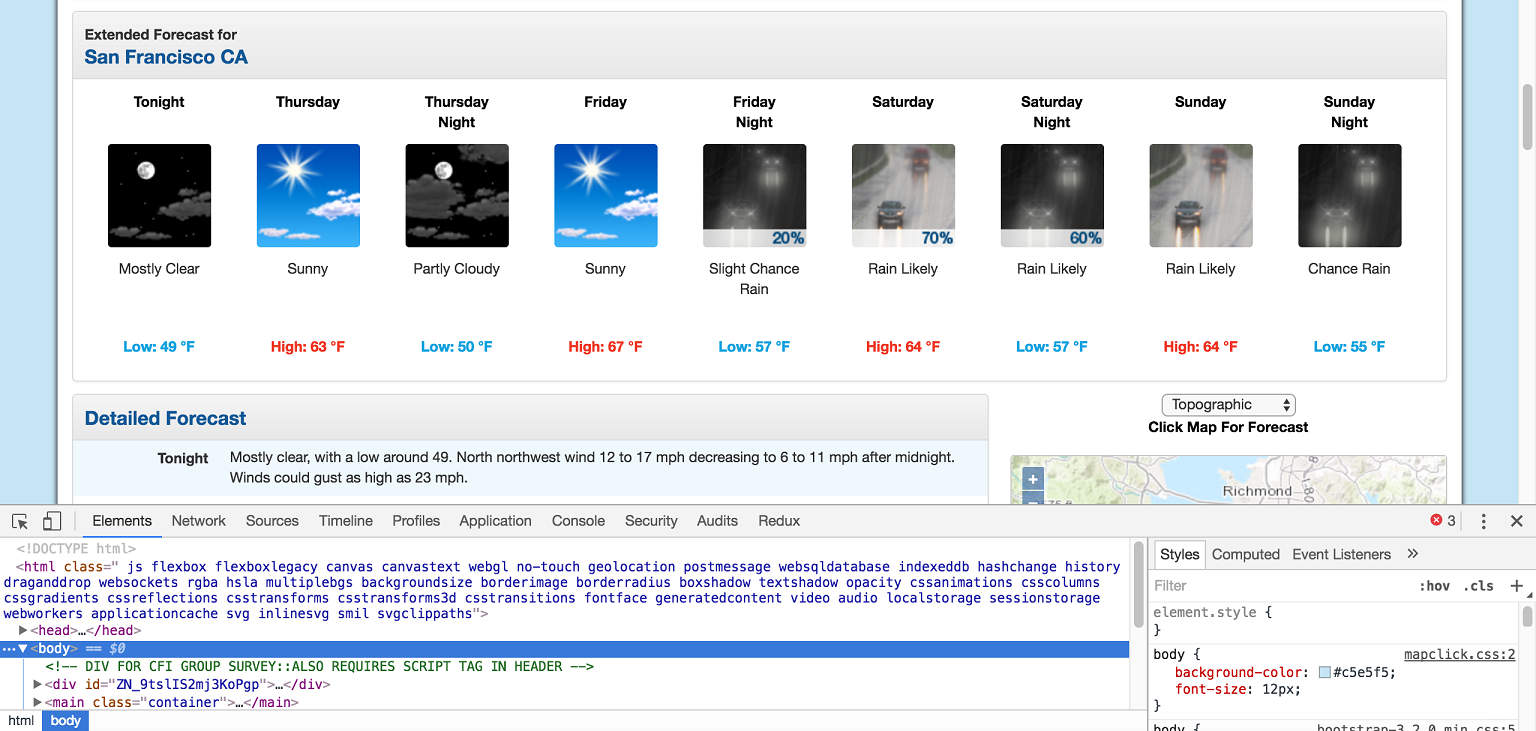
\includegraphics[width=0.9\linewidth,keepaspectratio]{bs41}
\end{center}
\end{frame}


%%%%%%%%%%%%%%%%%%%%%%%%%%%%%%%%%%%%%%%%%%%%%%%%%%%%%%%%%%%%%%%%%%%%%%%%%%%%%%%%%%%
\begin{frame}[fragile]\frametitle{Exploring page structure}
By right clicking on the page near where it says "Extended Forecast", then clicking "Inspect", we'll open up the tag that contains the text "Extended Forecast" in the elements panel:
	    \begin{center}
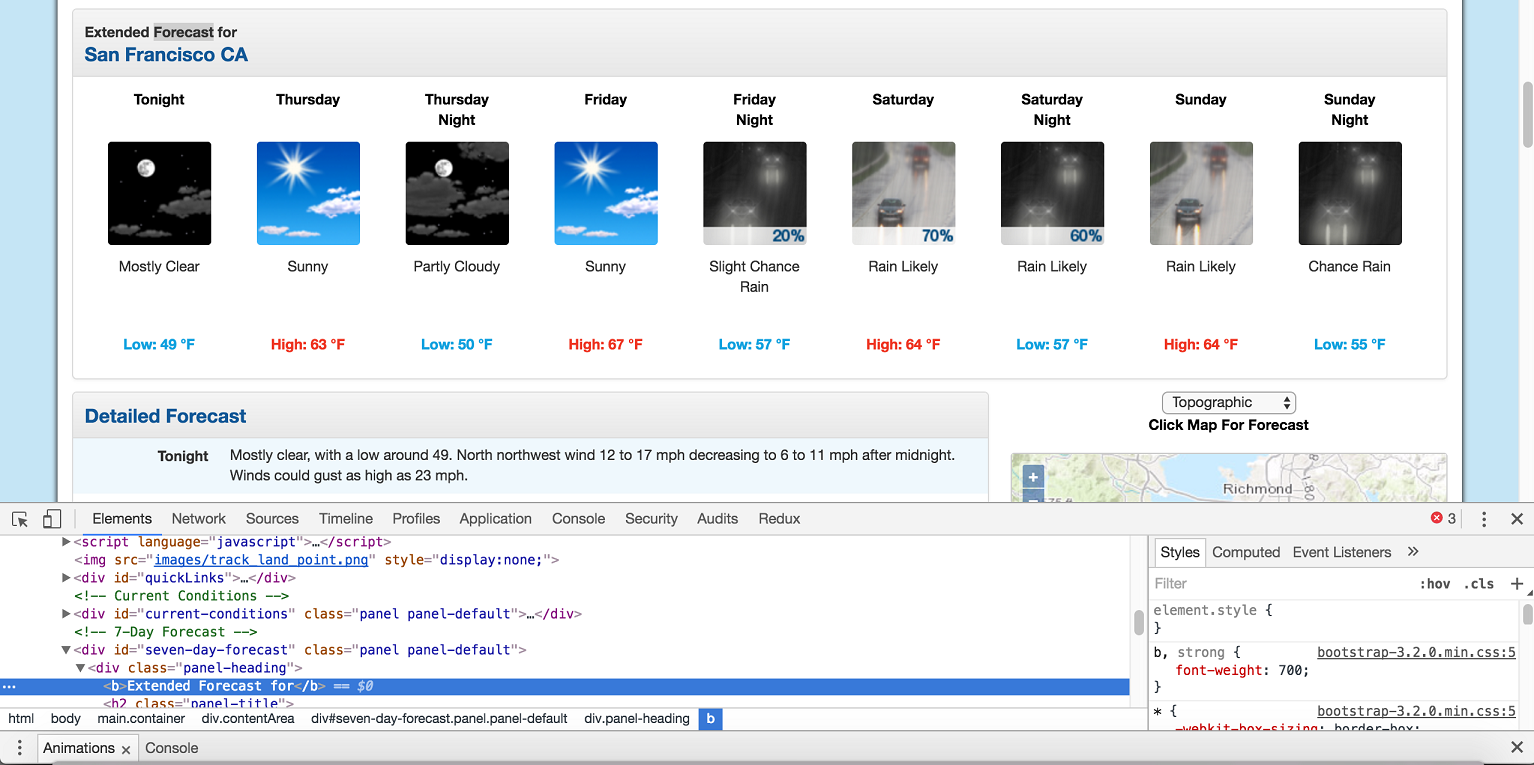
\includegraphics[width=0.9\linewidth,keepaspectratio]{bs42}
\end{center}
The extended forecast text.
\end{frame}

%%%%%%%%%%%%%%%%%%%%%%%%%%%%%%%%%%%%%%%%%%%%%%%%%%%%%%%%%%%%%%%%%%%%%%%%%%%%%%%%%%%
\begin{frame}[fragile]\frametitle{Exploring page structure}
We can then scroll up in the elements panel to find the "outermost" element that contains all of the text that corresponds to the extended forecasts. In this case, it's a div tag with the id seven-day-forecast:
	    \begin{center}
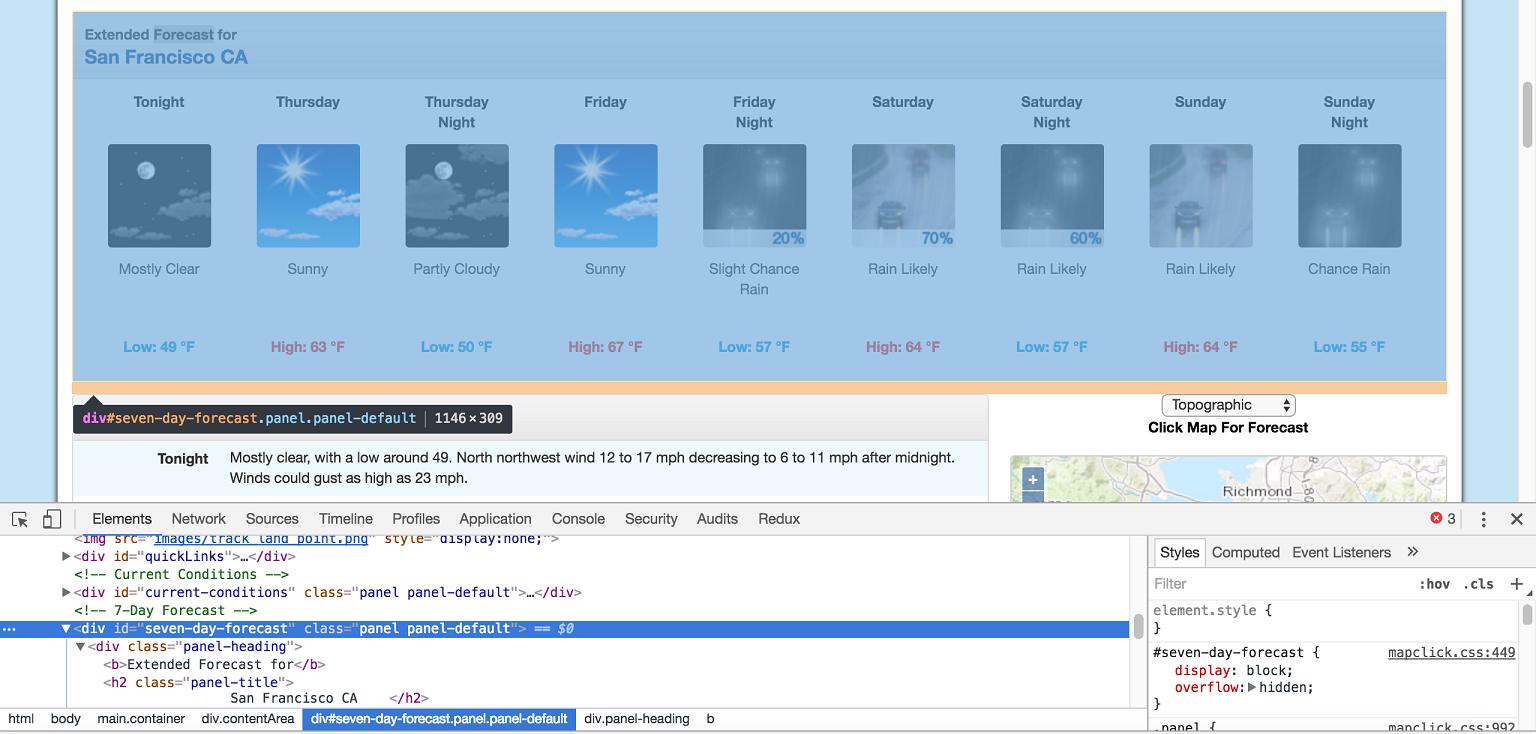
\includegraphics[width=0.9\linewidth,keepaspectratio]{bs43}
\end{center}
The div that contains the extended forecast items.
\end{frame}

%%%%%%%%%%%%%%%%%%%%%%%%%%%%%%%%%%%%%%%%%%%%%%%%%%%%%%%%%%%%%%%%%%%%%%%%%%%%%%%%%%%
\begin{frame}[fragile]\frametitle{Exploring page structure}
 If you click around on the console, and explore the div, you'll discover that each forecast item (like ``Tonight'', ``Thursday'', and ``Thursday Night'') is contained in a div with the class tombstone-container. Steps:
     \begin{itemize}
    \item     Download the web page containing the forecast.
    \item     Create a BeautifulSoup class to parse the page.
    \item     Find the div with id seven-day-forecast, and assign to seven\_day
    \item     Inside seven\_day, find each individual forecast item.
    \item     Extract and print the first forecast item.
	    \end{itemize}
\end{frame}


%%%%%%%%%%%%%%%%%%%%%%%%%%%%%%%%%%%%%%%%%%%%%%%%%%%%%%%%%%%%%%%%%%%%%%%%%%%%%%%%%%%
\begin{frame}[fragile]\frametitle{Get the data}

            \begin{lstlisting}
page = requests.get("http://forecast.weather.gov/MapClick.php?lat=37.7772\&lon=-122.4168")
soup = BeautifulSoup(page.content, 'html.parser')
seven_day = soup.find(id="seven-day-forecast")
forecast_items = seven_day.find_all(class_="tombstone-container")
tonight = forecast_items[0]
print(tonight.prettify())
\end{lstlisting}
\end{frame}


%%%%%%%%%%%%%%%%%%%%%%%%%%%%%%%%%%%%%%%%%%%%%%%%%%%%%%%%%%%%%%%%%%%%%%%%%%%%%%%%%%%
\begin{frame}[fragile]\frametitle{Get the data}

            \begin{lstlisting}
<div class="tombstone-container">
 <p class="period-name">
  Tonight
  <br>
   <br/>
  </br>
 </p>
 <p>
  <img alt="Tonight: Mostly clear, with a low around 49. West northwest wind 12 to 17 mph decreasing to 6 to 11 mph after midnight. Winds could gust as high as 23 mph. " class="forecast-icon" src="newimages/medium/nfew.png" title="Tonight: Mostly clear, with a low around 49. West northwest wind 12 to 17 mph decreasing to 6 to 11 mph after midnight. Winds could gust as high as 23 mph. "/>
 </p>
 <p class="short-desc">
  Mostly Clear
 </p>
 <p class="temp temp-low">
  Low: 49F
 </p>
</div>
\end{lstlisting}
\end{frame}

%%%%%%%%%%%%%%%%%%%%%%%%%%%%%%%%%%%%%%%%%%%%%%%%%%%%%%%%%%%%%%%%%%%%%%%%%%%%%%%%%%%
\begin{frame}[fragile]\frametitle{Extracting information from the page}
Inside the forecast item tonight is all the information we want. There are 4 pieces of information we can extract:
     \begin{itemize}
    \item     The name of the forecast item : in this case, Tonight.
    \item         The description of the conditions : this is stored in the title property of img.
    \item         A short description of the conditions : in this case, Mostly Clear.
    \item         The temperature low : in this case, 49 degrees.

	    \end{itemize}
	                \begin{lstlisting}
period = tonight.find(class_="period-name").get_text()
short_desc = tonight.find(class_="short-desc").get_text()
temp = tonight.find(class_="temp").get_text()

print(period)
print(short_desc)
print(temp)
\end{lstlisting}
\end{frame}


%%%%%%%%%%%%%%%%%%%%%%%%%%%%%%%%%%%%%%%%%%%%%%%%%%%%%%%%%%%%%%%%%%%%%%%%%%%%%%%%%%%
\begin{frame}[fragile]\frametitle{Extracting information from the page}
we can extract the title attribute from the img tag. To do this, we just treat the BeautifulSoup object like a dictionary, and pass in the attribute we want as a key:
	                \begin{lstlisting}
img = tonight.find("img")
desc = img['title']

print(desc)
Tonight: Mostly clear, with a low around 49. West northwest wind 12 to 17 mph decreasing to 6 to 11 mph after midnight. Winds could gust as high as 23 mph.
\end{lstlisting}
\end{frame}

%%%%%%%%%%%%%%%%%%%%%%%%%%%%%%%%%%%%%%%%%%%%%%%%%%%%%%%%%%%%%%%%%%%%%%%%%%%%%%%%%%%
\begin{frame}[fragile]\frametitle{Extracting all the information from the page}
Inside the forecast item tonight is all the information we want. There are 4 pieces of information we can extract:
     \begin{itemize}
    \item    Select all items with the class period-name inside an item with the class tombstone-container in seven\_day.
    \item        Use a list comprehension to call the get\_text method on each BeautifulSoup object.
	    \end{itemize}
	                \begin{lstlisting}
period_tags = seven_day.select(".tombstone-container .period-name")
periods = [pt.get_text() for pt in period_tags]
periods
['Tonight',
 'Thursday',
 'ThursdayNight',
 'Friday',
 'FridayNight',
 'Saturday',
 'SaturdayNight',
 'Sunday',
 'SundayNight']
\end{lstlisting}
Gets us each of the period names, in order.
\end{frame}


%%%%%%%%%%%%%%%%%%%%%%%%%%%%%%%%%%%%%%%%%%%%%%%%%%%%%%%%%%%%%%%%%%%%%%%%%%%%%%%%%%%
\begin{frame}[fragile]\frametitle{Extracting all the information from the page}
We can apply the same technique to get the other 3 fields:

	                \begin{lstlisting}
short_descs = [sd.get_text() for sd in seven_day.select(".tombstone-container .short-desc")]
temps = [t.get_text() for t in seven_day.select(".tombstone-container .temp")]
descs = [d["title"] for d in seven_day.select(".tombstone-container img")]

print(short_descs)
print(temps)
print(descs)

['Mostly Clear', 'Sunny' ... 'Rain Likely', 'Rain Likely', 'Chance Rain']
['Low: 49F', 'High: 63F' ... 'High: 64F', 'Low: 55F']
['Tonight: Mostly clear,...around 55.']
\end{lstlisting}
\end{frame}

%%%%%%%%%%%%%%%%%%%%%%%%%%%%%%%%%%%%%%%%%%%%%%%%%%%%%%%%%%%%%%%%%%%%%%%%%%%%%%%%%%%
\begin{frame}[fragile]\frametitle{Combining our data into a Pandas Dataframe}
We'll call the DataFrame class, and pass in each list of items that we have. We pass them in as part of a dictionary.

	                \begin{lstlisting}
import pandas as pd
weather = pd.DataFrame({
        "period": periods, 
        "short_desc": short_descs, 
        "temp": temps, 
        "desc":descs
    })

\end{lstlisting}
\end{frame}

%%%%%%%%%%%%%%%%%%%%%%%%%%%%%%%%%%%%%%%%%%%%%%%%%%%%%%%%%%%%%%%%%%%%%%%%%%%%%%%%%%%
\begin{frame}[fragile]\frametitle{Combining our data into a Pandas Dataframe}
We can now do some analysis on the data. For example, we can use a regular expression and the Series.str.extract method to pull out the numeric temperature values:

\begin{lstlisting}
temp_nums = weather["temp"].str.extract("(?P<temp_num>\d+)", expand=False)
weather["temp_num"] = temp_nums.astype('int')
temp_nums

0    49
1    63
2    50
3    67
4    57
5    64
6    57
7    64
8    55
\end{lstlisting}
\end{frame}

%%%%%%%%%%%%%%%%%%%%%%%%%%%%%%%%%%%%%%%%%%%%%%%%%%%%%%%%%%%%%%%%%%%%%%%%%%%%%%%%%%%
\begin{frame}[fragile]\frametitle{Combining our data into a Pandas Dataframe}
We could then find the mean of all the high and low temperatures:

\begin{lstlisting}
weather["temp_num"].mean()

58.444444444444443
\end{lstlisting}
We could also only select the rows that happen at night:
\begin{lstlisting}
is_night = weather["temp"].str.contains("Low")
weather["is_night"] = is_night
is_night

0     True
1    False
2     True
3    False
4     True
5    False
6     True
7    False
8     True
\end{lstlisting}
\end{frame}

%%%%%%%%%%%%%%%%%%%%%%%%%%%%%%%%%%%%%%%%%%%%%%%%%%%%%%%%%%%%%%%%%%%%%%%%%%%%%%%%%%%
\begin{frame}[fragile]\frametitle{Next Steps}
Some good examples of data to scrape are:
     \begin{itemize}
    \item        News articles
    \item         Sports scores
    \item         Weather forecasts
    \item         Stock prices
    \item         Online retailer prices


	    \end{itemize}
\end{frame}















